\documentclass[main.tex]{subfiles}


\begin{document}

%from pagenumber to up
% \phantomsection 
% \hypertarget{toc}{}

\pagestyle{empty}

\begin{NoHyper} % отключить клик-ссылки

% номер секции вручную
\setcounter{section}{15
}
\addtocounter{section}{-1} 

\section{Конденсатор}


% \sbox{0}{%
% 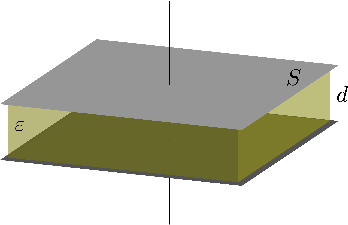
\includegraphics[]{el/15cap_pic.pdf}%
% }

% {%
% \setlength\intextsep{0pt}
% \begin{wrapfigure}[]{r}{\wd0}
%     \centering
%     \usebox{0}%
%     \caption{Плоский конденсатор}
%     \label{fig:p115}
% \end{wrapfigure}


\textbf{Конденсатор}~--- это устройство для накопления электрических зарядов. На рис.\,\ref{fig:p115} показана конструкция \emph{плоского конденсатора}.


    \begin{figure}[H]
    \centering
\begin{asy}
settings.outformat="png";
// settings.prc=true;
//settings.render=15;

import three;
import texcolors;
import x11colors;
size(6cm,0);
currentprojection =
orthographic((5,2,1.5));


//styles
///////////////////////////////////////////
DefaultHead3.size=new real(pen p=currentpen) {return 3mm;};
defaultpen(fontsize(11pt));
defaultpen(linewidth(0.4pt));
pen thick=black+2*linewidth(currentpen);
/////////////////////////////////////////


//draw(surface(path3D), lightgray+opacity(.5));
//draw(path3D, Chocolate+thick,L=Label("$S$",EndPoint,N,black));

//axes
//draw(O--2.5X,L=Label("$x$",EndPoint,WSW));
//draw(O--2.3Y,L=Label("$y$",EndPoint,ESE));
//draw(O--3Z,L=Label("$\vec n$",EndPoint,W),Arrow3(angle=10));
//draw(O--rotate(-30,X)*4Z,Green+thick,L=Label("$\vec B$",EndPoint,E,black),Arrow3(3.5mm,angle=10,emissive(Green)));

//draw("$\alpha$",reverse(arc(O,0.8*Z,rotate(-30,X)*0.8*Z)),N+0.3E);


//plate
real a=4.5;
path3 pl=((-a,-a,0)--(a,-a,0)--(a,a,0)--(-a,a,0)--cycle); 
draw(surface(pl), gray+opacity(1));

path3 pl=((-a,-a,0)--(a,-a,0)--(a,a,0)--(-a,a,0)--cycle); 
draw(shift(0,0,2)*surface(pl), lightgray+opacity(1));


//cube
transform3 sh=shift(-.5,-.5,0.025);
transform3 xsc=xscale3(1.9a);
transform3 ysc=yscale3(1.9a);
transform3 zsc=zscale3(1.9);

draw(zsc*ysc*xsc*sh*unitcube,yellow+opacity(.3));


//labels
//dot((.95a,-.95a,1));

label(Label("$\varepsilon$"),(a,-.93a,1.25),E);
label(Label("$d$"),(-.95a,.95a,1),E);
label(Label("$S$"),(-.15a,.97a,2),N);


//outputs
draw((0,0,2)--5Z);
draw((0,0,0)--(-3Z));


    
\end{asy}
\caption{Плоский конденсатор}
\label{fig:p115}
\end{figure}


Простейший плоский конденсатор состоит из двух параллельных металлических пластин (\emph{обкладки}) площадью~$S$ каждая, расположенных на малом расстоянии~$d$ друг от друга и разделенных слоем диэлектрика\footnote{Также между обкладками может быть \emph{вакуум} ($\varepsilon=1$). Диэлектрическая проницаемость \emph{воздуха} обычно также считается равной единице.} с диэлектрической проницаемостью~$\varepsilon$. 
Конденсатор также имеет \emph{выводы} (черные линии на рис.\,\ref{fig:p115}) для его соединения с другими устройствами. 

Обычно в заряженном конденсаторе (то есть накопившем заряды на своих обкладках) одна из пластин конденсатора несет заряд~$+q$, а другая~--- заряд~$-q$. Под \emph{зарядом конденсатора} понимают заряд его \emph{положительной} обкладки.

\textbf{Емкость} ($C$ [Ф])~--- это характеристика конденсатора, показывающая его способность накапливать заряд:
\begin{equation}
    C=\frac{q}{U},
\end{equation}
где $q$~--- заряд конденсатора,
% \footnote{Обычно одна из пластин конденсатора несет заряд~$+q$, а другая~--- заряд $-q$.},
$U$~--- напряжение между пластинами.

Емкость численно равна заряду конденсатора при напряжении 1~В между его обкладками. 

\textbf{Емкость конденсатора} зависит от его размеров и диэлектрика в нем:
\begin{equation}
    C=\frac{\varepsilon\varepsilon_0S}{d},
\end{equation}
где $\varepsilon_0$~--- электрическая постоянная (см.~справочные таблицы).

\textbf{Энергия конденсатора} рассчитывается по формуле:
\begin{equation}
    W_C=\frac{CU^2}{2}.
\end{equation}

% \medskip

\noindent\textbf{Задача.} Плоский конденсатор состоит из двух параллельно расположенных в воздухе пластинок, каждая площадью 100~см$^2$, расстояние между ними 0,2~см. Определите емкость конденсатора.

\smallskip

\noindent\emph{Решение}. Между пластинами воздух: $\varepsilon=1$. Электрическая постоянная $\varepsilon_0\hm\approx8{,}85\cdot10^{-12}$~Ф/м. Тогда:
\begin{equation*}
    C=\frac{\varepsilon\varepsilon_0S}{d}=\frac{1\cdot8{,}85\cdot10^{-12}\cdot100\cdot10^{-4}}{0{,}2\cdot10^{-2}}=4{,}425\cdot10^{-11}~\text{Ф}.
\end{equation*}














\end{NoHyper}
\end{document}
